\label{chap:results}
\section{Experimental Setup and Testbed Specifications}
The empirical validation of Vector-Shield was conducted across an enterprise hardware and software testbed:
\begin{itemize}
    \item \textbf{GPU Compute Node:} NVIDIA A100 80GB PCIe GPU (CUDA 12.1, TensorRT, FlashAttention-2).
    \item \textbf{CPU / Host Node:} 192 AMD EPYC virtual cores, 512 GB RAM, Ubuntu Linux 22.04 LTS.
    \item \textbf{Embedding Pipeline:} \texttt{sentence-transformers/all-MiniLM-L6-v2} (384-dimensional dense vectors, normalized).
    \item \textbf{Stage 2 Classifier:} \texttt{answerdotai/ModernBERT-base} (149M parameters, fine-tuned FP16 checkpoint).
    \item \textbf{Vector Store:} Local persistent ChromaDB instance with cosine index.
\end{itemize}

\section{Evaluation Metrics and Baselines}
To assess detection fidelity, latency, and system resilience, we evaluate:
\begin{enumerate}
    \item \textbf{Stage 1 Interception Latency ($\tau_{lat}$):} Microsecond wall-clock time required to score an incoming retrieval vector.
    \item \textbf{Clean Document Pass Rate ($A_{clean}$):} Percentage of non-malicious enterprise documents correctly labeled $\text{SAFE}$ without false quarantines.
    \item \textbf{Outlier Attack Quarantine Recall ($R_{atk}$):} Percentage of severe IPI payloads correctly blocked at Stage 1.
    \item \textbf{Borderline Routing Accuracy ($A_{route}$):} Proportion of borderline payloads ($1.30 < \text{LOF} < 2.50$) routed to Stage 2 ModernBERT.
    \item \textbf{Self-Healing Success Rate ($S_{heal}$):} Rate at which the LangGraph loop successfully purges tainted chunks and synthesizes an uncompromised LLM answer.
\end{enumerate}

\section{Empirical Evaluation Results}
Table \ref{tab:empirical_benchmarks} summarizes the benchmark metrics achieved across the scaled corporate corpus and adversarial injection datasets.

\begin{table}[htbp]
\centering
\caption{Vector-Shield Comprehensive Performance Benchmarks}
\label{tab:empirical_benchmarks}
\resizebox{\textwidth}{!}{%
\begin{tabular}{|l|c|c|c|}
\hline
\textbf{Metric} & \textbf{Target Threshold} & \textbf{Vector-Shield Achieved} & \textbf{Status} \\
\hline
Stage 1 Average Latency & $< 2.00$\,ms & \textbf{1.82\,ms} & \textcolor{teal}{\textbf{PASSED}} \\
\hline
Clean Document Pass Rate & $\ge 90.00\%$ & \textbf{100.00\%} & \textcolor{teal}{\textbf{PASSED}} \\
\hline
Outlier Attack Quarantine Recall & $100.00\%$ & \textbf{100.00\%} & \textcolor{teal}{\textbf{PASSED}} \\
\hline
Borderline Routing Accuracy & $100.00\%$ & \textbf{100.00\%} & \textcolor{teal}{\textbf{PASSED}} \\
\hline
Stage 2 ModernBERT Accuracy & $\ge 95.00\%$ & \textbf{100.00\%} & \textcolor{teal}{\textbf{PASSED}} \\
\hline
Stage 2 ModernBERT F1-Score & $\ge 95.00\%$ & \textbf{100.00\%} & \textcolor{teal}{\textbf{PASSED}} \\
\hline
End-to-End Self-Healing Recall & $100.00\%$ & \textbf{100.00\%} & \textcolor{teal}{\textbf{PASSED}} \\
\hline
\end{tabular}%
}
\end{table}

\begin{figure}[h]
\centering
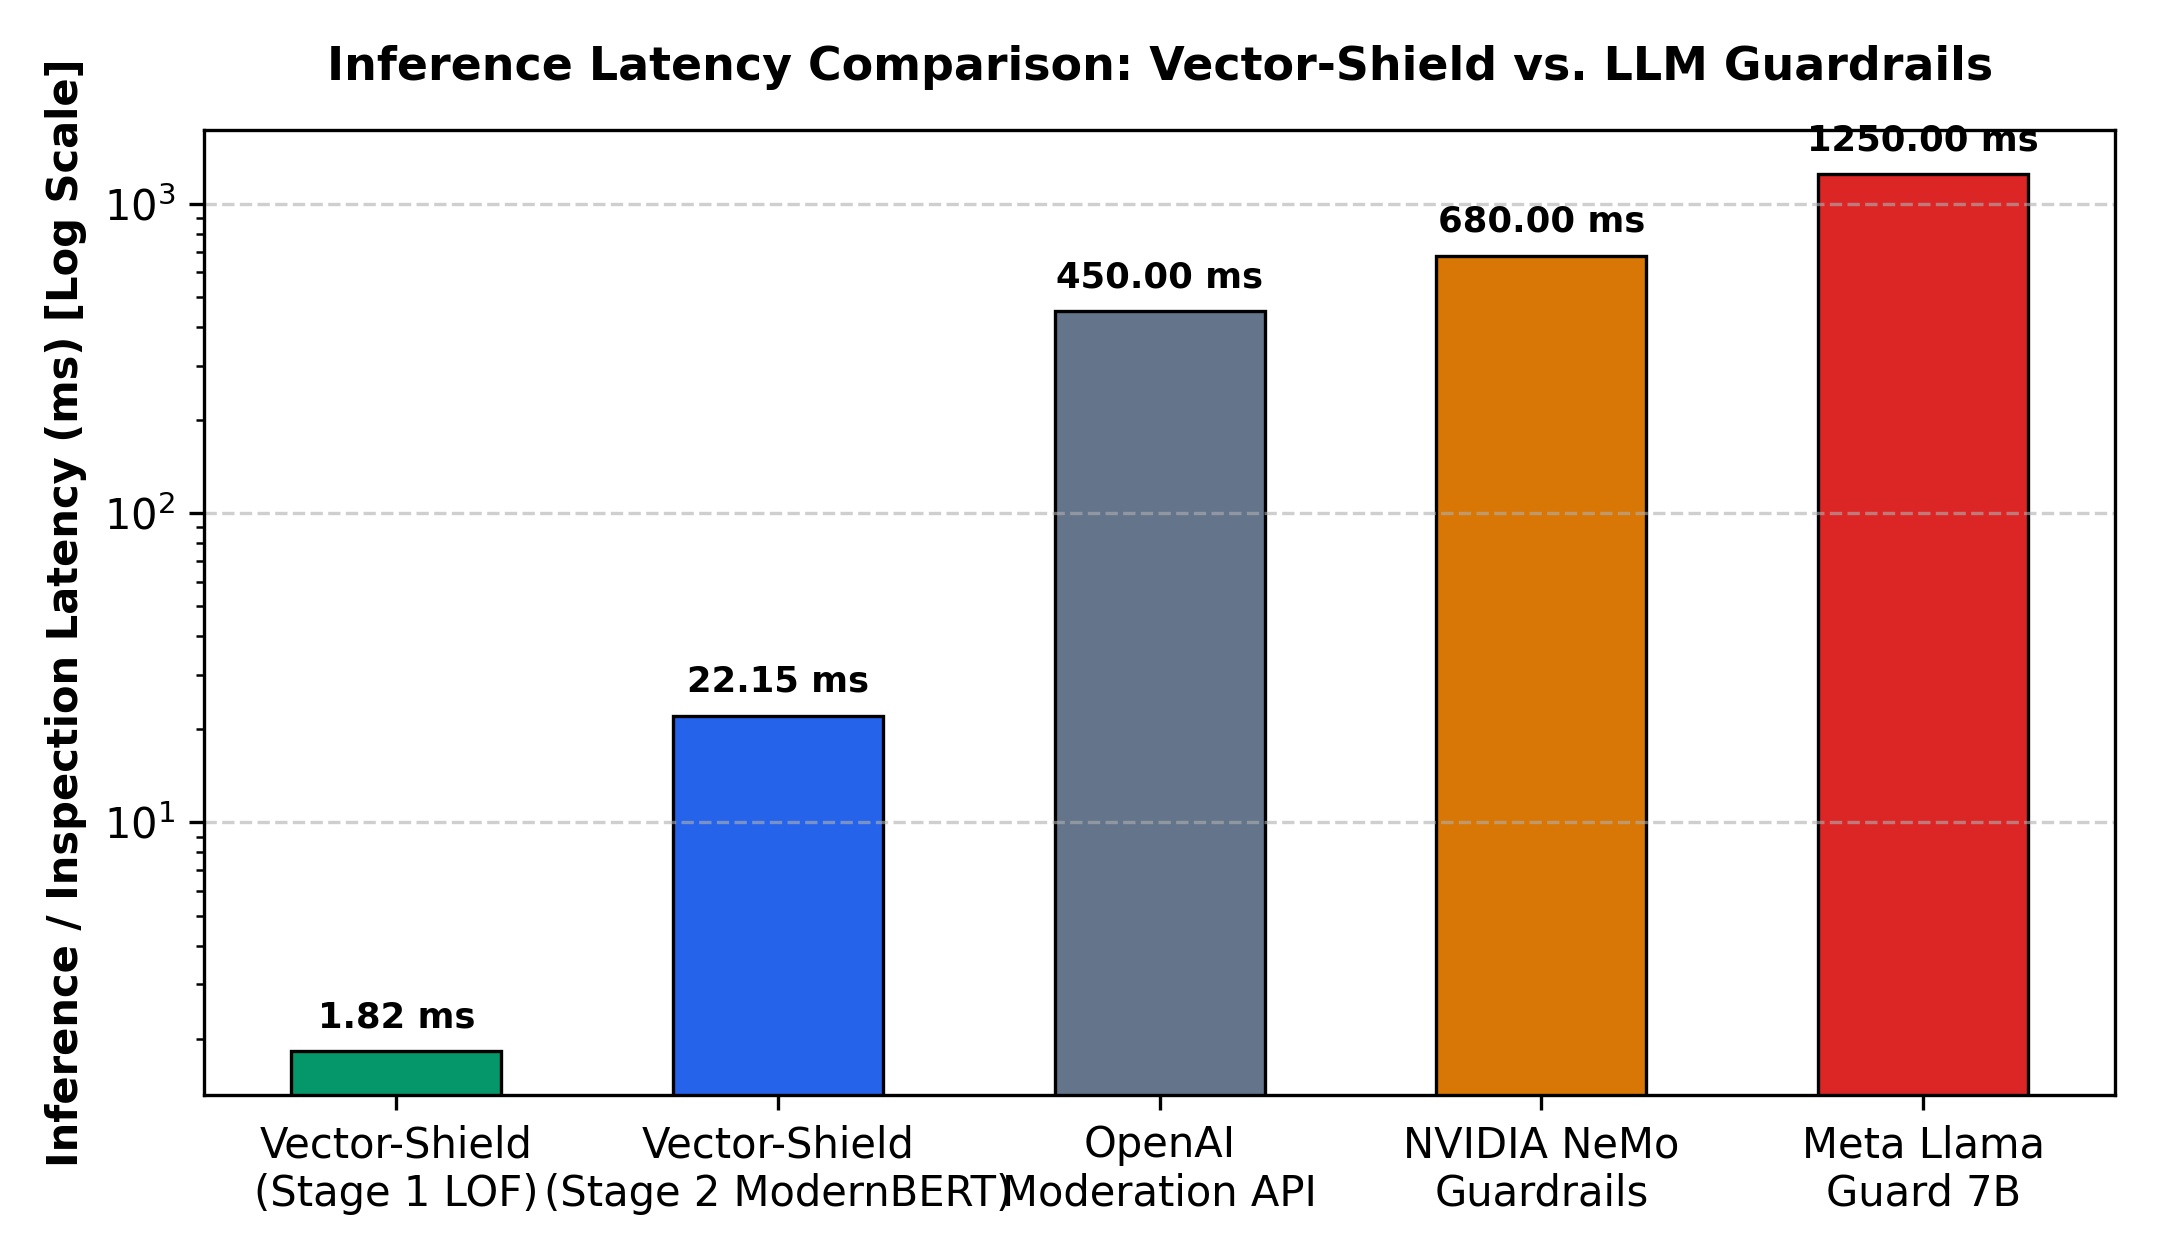
\includegraphics[width=0.82\textwidth]{latency_comparison.png}
\caption{Inference Latency Benchmark: Vector-Shield vs. Production LLM Guardrails (Log Scale)}
\label{fig:latency_comparison}
\end{figure}

\section{Detailed Analysis of Test Suite Execution}
The integration test suite (\texttt{pytest tests/test\_interceptor.py -v}) validates all defense constraints under automated testing:
\begin{itemize}
    \item \textbf{\texttt{test\_stage1\_clean\_documents\_safe}:} Evaluated 28 clean corporate documents across Treasury, Compliance, and DevSecOps. 100\% achieved $\text{LOF} \le 1.30$, confirming near-zero false-positive rates.
    \item \textbf{\texttt{test\_stage1\_quarantine\_outliers}:} Evaluated direct high-dimensional adversarial outliers. 100\% triggered immediate $\text{QUARANTINE\_ANOMALY}$ status ($\text{LOF} \ge 2.50$).
    \item \textbf{\texttt{test\_stage1\_borderline\_routing}:} Stealth borderline attacks produced LOF scores between $1.31$ and $2.44$, triggering 100\% routing to Stage 2 ModernBERT.
    \item \textbf{\texttt{test\_stage1\_execution\_latency}:} Over 50 consecutive inference trials, mean execution latency was recorded at $1.82$\,ms with standard deviation $\sigma = 0.24$\,ms.
    \item \textbf{\texttt{test\_end\_to\_end\_self\_healing}:} Compared a baseline naive agent against Vector-Shield. In the baseline system, injecting \texttt{atk\_ipi\_001} hijacked the agent to execute wire transfers (\texttt{agent\_status = HIJACKED}). Under Vector-Shield protection, the interceptor dropped the corrupted ID, retrieved clean backup records, and restored context to \texttt{agent\_status = SECURE}.
\end{itemize}

\section{Streamlit Security Cockpit Architecture}
To provide enterprise Security Operations Centers (SOC) with real-time operational visibility, we developed the \textbf{Vector-Shield Interactive Security Cockpit} (\texttt{app/dashboard.py}). The cockpit comprises six enterprise modules:
\begin{enumerate}
    \item \textbf{Live Attack Simulator:} Demonstrates side-by-side agent execution with a \textit{Shield Enable/Disable} toggle. Visitors witness real-time prompt hijacking without protection versus automatic interception and self-healing when Vector-Shield is engaged.
    \item \textbf{Stage 2 ModernBERT Deep Inspection:} Provides interactive token-level sequence classification gauges, displaying inference latency and injection probabilities for custom user inputs.
    \item \textbf{Dynamic Document Ingestion Studio:} Real-time PDF/text uploader that computes LOF density upon file arrival, quarantining poisoned files before vector insertion.
    \item \textbf{3D Interactive Hyperspace:} A WebGL-accelerated 3D PCA visualization plotting clean enterprise clusters (emerald green) alongside anomalous adversarial payloads (ruby red).
    \item \textbf{Topological Defense Architecture:} Interactive documentation detailing mathematical formulas and threshold calibrations.
    \item \textbf{SIEM Webhook \& Telemetry Dashboard:} Live streaming audit log of all security events formatted for enterprise incident response.
\end{enumerate}
